\begin{figure}
  \centering
  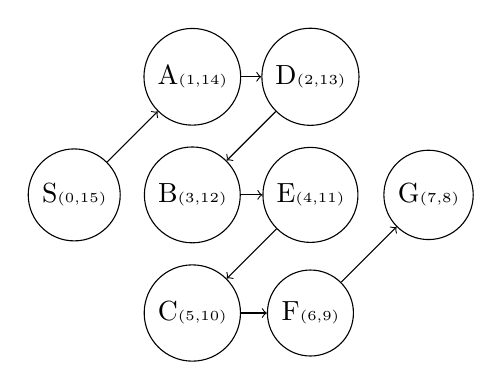
\begin{tikzpicture}[->, auto, node distance=1.5cm, every node/.style={circle, draw, minimum size=.5cm}]
    \node (S) {S\tiny{(0,15)}};
    \node (B) [right of=S] {B\tiny{(3,12)}};
    \node (A) [above of=B] {A\tiny{(1,14)}};
    \node (C) [below of=B] {C\tiny{(5,10)}};
    \node (D) [right of=A] {D\tiny{(2,13)}};
    \node (E) [below of=D] {E\tiny{(4,11)}};
    \node (F) [below of=E] {F\tiny{(6,9)}};
    \node (G) [right of=E] {G\tiny{(7,8)}};

    \path[every node]
    (S) edge (A)
    (A) edge (D)
    (D) edge (B)
    (B) edge (E)
    (E) edge (C)
    (C) edge (F)
    (F) edge (G)
    ;
  \end{tikzpicture}

  \caption{Tiefensuchwald}\label{fig:dfstree}
\end{figure}